\documentclass[aspectratio=169]{beamer}
\usetheme{Madrid}
\usepackage{amsmath,amssymb,booktabs,tikz}
\usetikzlibrary{arrows.meta}
\definecolor{ufblue}{HTML}{003087}
\definecolor{uforange}{HTML}{FA4616}
\definecolor{stagegreen}{HTML}{007766}
\setbeamercolor{structure}{fg=ufblue}
\setbeamertemplate{navigation symbols}{}
\setbeamertemplate{footline}[frame number]
\title{Runge--Kutta Methods}
\subtitle{Geometry, slope averages, and the path to RK4}
\author{Dr. Harrington}
\institute{MAD 4401 --- University of Florida}
\date{}
% All diagrams are native TikZ. Compile twice with pdflatex.
% k_i denotes a slope, not an increment h*f.
\newcommand{\axes}{
\draw[->] (-.08,.75)--(1.25,.75) node[right]{$t$};
\draw[->] (0,.75)--(0,3.2) node[above]{$y$};
\foreach \x in {.5,1}{\draw (\x,.72)--(\x,.78) node[below=3pt] {\scriptsize\x};}
\foreach \y in {1,2,3}{\draw (-.015,\y)--(.015,\y) node[left=3pt]{\scriptsize\y};}
\draw[gray,dotted] (1,.8)--(1,3.05);
}
\newcommand{\expcurve}{\draw[black,thick,domain=0:1.04,samples=50] plot(\x,{exp(\x)});}
\newcommand{\stageplot}[1]{
\begin{tikzpicture}[x=4.5cm,y=1.65cm,>=Stealth]
\axes\expcurve
\fill (0,1) circle(1.5pt);
\draw[ufblue,thick,->] (0,1)--(.5,1.5);
\fill[ufblue] (.5,1.5) circle(1.6pt);
\node[ufblue,right] at (.51,1.43){\scriptsize $P_2$};
\ifnum#1>1
\draw[uforange,thick,->] (0,1)--(.5,1.75);
\fill[uforange] (.5,1.75) circle(1.6pt);
\node[uforange,left] at (.49,1.8){\scriptsize $P_3$};
\fi
\ifnum#1>2
\draw[stagegreen,thick,->] (0,1)--(1,2.75);
\fill[stagegreen] (1,2.75) circle(1.6pt);
\node[stagegreen,right] at (1,2.86){\scriptsize $P_4$};
\fi
\end{tikzpicture}}
\begin{document}
\frame{\titlepage}
\begin{frame}{Methods we already know}
For $y'=f(t,y)$, approximate $y(t_n)$ by $y_n$.
\begin{align*}
\text{Euler:}\quad y_{n+1}&=y_n+h f(t_n,y_n),\\
\text{Improved Euler:}\quad y_{n+1}&=y_n+\frac h2\bigl[f(t_n,y_n)+f(t_n+h,y_n+hf(t_n,y_n))\bigr].
\end{align*}
Taylor methods add higher derivatives of the solution:
\[y(t_n+h)=y(t_n)+hy'(t_n)+\frac{h^2}{2}y''(t_n)+\cdots.\]
\textbf{Runge--Kutta idea:} obtain higher accuracy by evaluating $f$ at carefully chosen trial points.
\end{frame}
\begin{frame}{A geometric starting example}
\begin{columns}
\column{.48\textwidth}
\[y'=1+2t,\quad y(0)=1,\quad h=1.\]
The exact solution is $y(t)=1+t+t^2$.
\[k_1=f(0,1)=1.\]
Euler follows the initial slope:
\[y_1=1+1(1)=2.\]
The exact endpoint is $y(1)=3$.
\column{.48\textwidth}
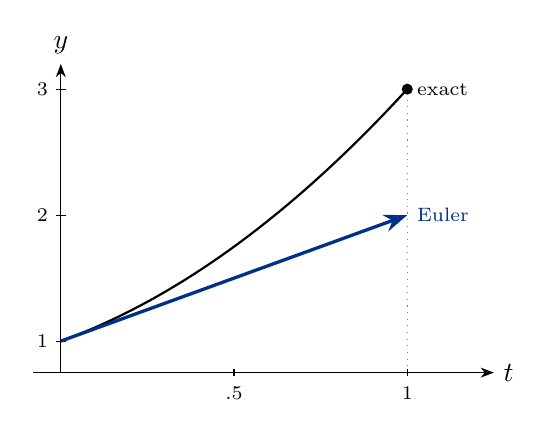
\begin{tikzpicture}[x=4.4cm,y=1.6cm,>=Stealth]
\axes
\draw[black,thick,domain=0:1,samples=40] plot(\x,{1+\x+\x*\x});
\draw[ufblue,very thick,->] (0,1)--(1,2);
\fill (1,3) circle(2pt) node[right]{\scriptsize exact};
\node[ufblue,right] at (1,2){\scriptsize Euler};
\end{tikzpicture}
\end{columns}
\end{frame}
\begin{frame}{The weights come from an average slope}
\begin{columns}
\column{.48\textwidth}
Here the slope is $g(t)=1+2t$.
\[y(1)-y(0)=\int_0^1g(t)\,dt.\]
The trapezoid has area
\[1\cdot\frac{1+3}{2}=2.\]
Thus the average slope is
\[\boxed{\overline{k}=\tfrac12 k_1+\tfrac12 k_2=2}.\]
The update is $y_1=1+1(2)=3$.
\column{.48\textwidth}
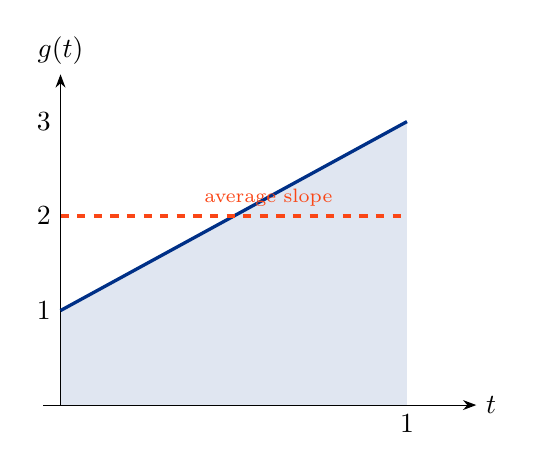
\begin{tikzpicture}[x=4.4cm,y=1.2cm,>=Stealth]
\fill[ufblue!12] (0,0)--(1,0)--(1,3)--(0,1)--cycle;
\draw[->] (-.05,0)--(1.2,0) node[right]{$t$};
\draw[->] (0,0)--(0,3.5) node[above]{$g(t)$};
\draw[ufblue,very thick] (0,1)--(1,3);
\draw[uforange,very thick,dashed] (0,2)--(1,2);
\node[left] at (0,1){$1$};\node[left] at (0,2){$2$};\node[left] at (0,3){$3$};
\node[below] at (1,0){$1$};
\node[uforange,above] at (.6,2){\scriptsize average slope};
\end{tikzpicture}
\end{columns}
\medskip
Equal endpoint weights integrate a linear slope exactly.
\end{frame}
\begin{frame}{Improved Euler for a general ODE}
Along the exact solution,
\[y(t_n+h)-y(t_n)=\int_{t_n}^{t_n+h}f(t,y(t))\,dt.\]
A trapezoid approximation would use both endpoint slopes, but the final solution value is unknown. Use an Euler predictor:
\begin{align*}
k_1&=f(t_n,y_n), & \widetilde y_{n+1}&=y_n+hk_1,\\
k_2&=f(t_n+h,\widetilde y_{n+1}), &
y_{n+1}&=y_n+h\left(\tfrac12 k_1+\tfrac12 k_2\right).
\end{align*}
\textbf{Improved Euler is an RK2 method.} The second slope comes from a trial endpoint. For general $f(t,y)$, it is only an estimate of the exact endpoint slope.
\end{frame}
\begin{frame}{When the slope depends on the height}
\begin{columns}
\column{.49\textwidth}
\[y'=y,\quad y(0)=1,\quad h=1.\]
\[k_1=1,\quad \widetilde y_1=2,\quad k_2=f(1,2)=2.\]
\[y_1=1+\tfrac12(1+2)=2.5.\]
The second slope is evaluated at $(1,2)$, below the exact solution $e^t$.
\medskip
We use a large step to make the geometry visible.
\column{.47\textwidth}
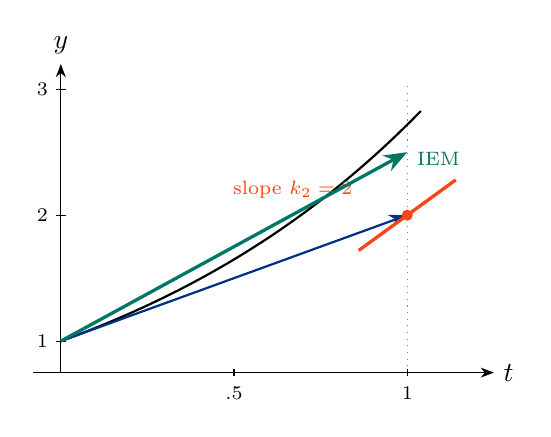
\begin{tikzpicture}[x=4.4cm,y=1.6cm,>=Stealth]
\axes\expcurve
\draw[ufblue,thick,->] (0,1)--(1,2);
\draw[uforange,very thick] (.86,1.72)--(1.14,2.28);
\fill[uforange] (1,2) circle(2pt);
\node[uforange,left] at (.87,2.2){\scriptsize slope $k_2=2$};
\draw[stagegreen,very thick,->] (0,1)--(1,2.5);
\node[stagegreen,right] at (1,2.45){\scriptsize IEM};
\end{tikzpicture}
\end{columns}
\end{frame}
\begin{frame}{The geometry of the equal weights}
\begin{columns}
\column{.48\textwidth}
Translate both sampled slopes to the starting point $(0,1)$.
\[1+hk_1=2,\qquad 1+hk_2=3.\]
The averaged slope reaches the midpoint of these two heights:
\[\tfrac12(2)+\tfrac12(3)=2.5.\]
\textbf{We average slopes, not angles.}
The translated $k_2$ line illustrates the average. We still evaluate $k_2$ at $(1,2)$.
\column{.48\textwidth}
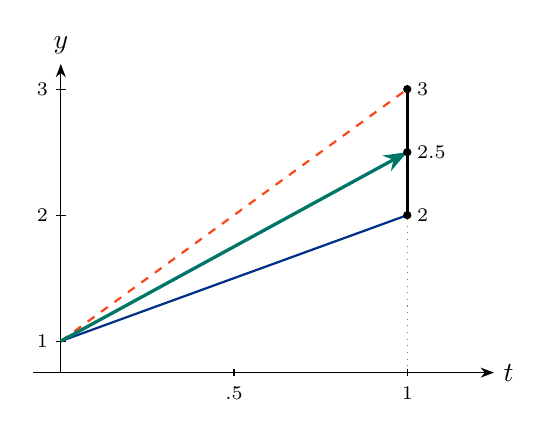
\begin{tikzpicture}[x=4.4cm,y=1.6cm,>=Stealth]
\axes
\draw[ufblue,thick] (0,1)--(1,2);
\draw[uforange,thick,dashed] (0,1)--(1,3);
\draw[stagegreen,very thick,->] (0,1)--(1,2.5);
\draw[very thick] (1,2)--(1,3);
\foreach \y in {2,2.5,3}{\fill (1,\y) circle(1.5pt);}
\node[right] at (1,2){\scriptsize $2$};
\node[right] at (1,2.5){\scriptsize $2.5$};
\node[right] at (1,3){\scriptsize $3$};
\end{tikzpicture}
\end{columns}
\end{frame}
\begin{frame}{Midpoint RK2 samples halfway through the step}
\begin{columns}
\column{.49\textwidth}
For the same example $y'=y$:
\[k_1=1,\quad P_2=(\tfrac12,1+\tfrac12 k_1)=(\tfrac12,1.5).\]
\[k_2=f(\tfrac12,1.5)=1.5.\]
Use this slope for the full step:
\[y_1=1+1(1.5)=2.5.\]
The weights are $(b_1,b_2)=(0,1)$. The first slope still determines the trial point.
\column{.47\textwidth}
\stageplot{1}
\end{columns}
\end{frame}
\begin{frame}{A family of two-stage methods}
Choose a fraction $c>0$ of the step for the second sample:
\begin{align*}
k_1&=f(t_n,y_n),\\
k_2&=f(t_n+ch,\ y_n+ch k_1),\\
y_{n+1}&=y_n+h(b_1k_1+b_2k_2).
\end{align*}
\begin{itemize}
\item $c$ chooses the location of the trial point along the Euler line.
\item $b_1,b_2$ choose the contributions to the final slope.
\end{itemize}
\textbf{These choices must work together to obtain second-order accuracy.}
\end{frame}
\begin{frame}{Geometric conditions on the weights}
Write $s=(t-t_n)/h$. A constant slope must remain unchanged:
\[\boxed{b_1+b_2=1}.\]
For a slope varying linearly as $g(s)=A+Bs$, its average on $[0,1]$ is $A+B/2$. The two samples give
\[b_1g(0)+b_2g(c)=(b_1+b_2)A+b_2cB.\]
Thus the weighted sample locations must have their average at the midpoint:
\[\boxed{b_2c=\tfrac12},\qquad
b_2=\frac{1}{2c},\quad b_1=1-\frac{1}{2c}.\]
Next we check why these same conditions work when $f$ depends on $y$.
\end{frame}
\begin{frame}{The connection to the Taylor method}
Start a step with exact input. Evaluate $f,f_t,f_y$ at $(t_n,y_n)$.
\[y''=\frac{d}{dt}f(t,y(t))=f_t+f_yf.\]
The exact expansion is
\[y(t_n+h)=y_n+hf+\frac{h^2}{2}(f_t+f_yf)+O(h^3).\]
The second stage has expansion
\[k_2=f(t_n+ch,y_n+chf)=f+ch(f_t+f_yf)+O(h^2).\]
Therefore the RK update is
\[y_{n+1}=y_n+h(b_1+b_2)f+h^2b_2c(f_t+f_yf)+O(h^3).\]
Matching coefficients gives $b_1+b_2=1$ and $b_2c=1/2$.
\end{frame}
\begin{frame}{Different samples, different weights, same order}
\renewcommand{\arraystretch}{1.6}
\begin{center}
\begin{tabular}{lccc}
\toprule Method & $c$ & $b_1$ & $b_2$\\\midrule
Improved Euler & $1$ & $1/2$ & $1/2$\\
Midpoint & $1/2$ & $0$ & $1$\\
Ralston RK2 & $2/3$ & $1/4$ & $3/4$\\\bottomrule
\end{tabular}
\end{center}
Each method has a one-step error $O(h^3)$ and global error $O(h^2)$ under the usual smoothness and Lipschitz assumptions.
\medskip
Their errors need not be equal. The agreement for $y'=y$ is a special feature of that example.
\end{frame}
\begin{frame}{What RK2 leaves out}
For $y'=y$, any member of this RK2 family gives
\[y_{n+1}=y_n\left(1+h+\frac{h^2}{2}\right).\]
But the exact step is
\[y(t_n+h)=y(t_n)\left(1+h+\frac{h^2}{2}+\frac{h^3}{6}+\frac{h^4}{24}+\cdots\right).\]
Taylor methods compute higher derivatives explicitly.
\medskip
\textbf{RK4 uses four coordinated slope evaluations to match through fourth order.} Additional slopes alone do not guarantee a higher order.
\end{frame}
\begin{frame}{RK4: the first midpoint trial}
\begin{columns}
\column{.49\textwidth}
Continue with $y'=y$, $y(0)=1$, $h=1$.
\[k_1=f(0,1)=1.\]
Move halfway along the first slope:
\[P_2=(\tfrac12,1+\tfrac12 k_1)=(\tfrac12,1.5).\]
\[\boxed{k_2=f(P_2)=1.5}.\]
The black curve is $e^t$. The blue arrow constructs the trial point.
\column{.47\textwidth}\stageplot{1}
\end{columns}
\end{frame}
\begin{frame}{RK4: a revised midpoint trial}
\begin{columns}
\column{.49\textwidth}
Use $k_2$ to form another trial point, measured from the original start:
\[P_3=(\tfrac12,1+\tfrac12 k_2)=(\tfrac12,1.75).\]
\[\boxed{k_3=f(P_3)=1.75}.\]
Both midpoint trials have the same time coordinate but different heights.
\medskip
We evaluate $f$ again because the height can affect the slope.
\column{.47\textwidth}\stageplot{2}
\end{columns}
\end{frame}
\begin{frame}{RK4: an endpoint trial}
\begin{columns}
\column{.49\textwidth}
Use the revised midpoint slope for a full trial step from $(0,1)$:
\[P_4=(1,1+k_3)=(1,2.75).\]
\[\boxed{k_4=f(P_4)=2.75}.\]
The trial endpoint supplies one more slope. The final answer will combine all four slopes.
\column{.47\textwidth}\stageplot{3}
\end{columns}
\end{frame}
\begin{frame}{RK4: the final weighted slope}
\[\overline{k}=\frac16k_1+\frac13k_2+\frac13k_3+\frac16k_4.\]
For our example,
\[\overline{k}=\frac{1+2(1.5)+2(1.75)+2.75}{6}=\frac{41}{24}.\]
\[\boxed{y_1=1+\overline{k}=\frac{65}{24}\approx2.708333}.\]
The trial endpoint was $2.75$. The exact endpoint is $e\approx2.718282$.
\medskip
The weights sum to $1$. Each midpoint slope receives twice the weight of either endpoint slope.
\end{frame}
\begin{frame}{The classical RK4 algorithm}
\begin{align*}
k_1&=f(t_n,y_n),\\
k_2&=f\left(t_n+\frac h2,y_n+\frac h2k_1\right),\\
k_3&=f\left(t_n+\frac h2,y_n+\frac h2k_2\right),\\
k_4&=f(t_n+h,y_n+hk_3),\\[2pt]
\boxed{y_{n+1}}&\boxed{=y_n+\frac h6(k_1+2k_2+2k_3+k_4)}.
\end{align*}
Every trial height is measured from $y_n$. Here the $k_i$ are slopes, so the update multiplies their weighted average by $h$.
\end{frame}
\begin{frame}{A geometric explanation for the RK4 weights}
First consider $y'=g(t)$, so trial heights do not affect the slopes.
The sample times are $0,1/2,1/2,1$ in normalized coordinates.
\medskip
Choose symmetric weights $(a,b,b,a)$. Matching the average of $1$ and $s^2$ on $[0,1]$ gives
\[2a+2b=1,\qquad \frac b2+a=\frac13.\]
Solving yields $a=1/6$ and $b=1/3$. These weights also integrate $s$ and $s^3$ exactly.
\[\frac16 g(t_n)+\frac23 g(t_n+h/2)+\frac16 g(t_n+h)\]
This is Simpson's average-slope formula. For general $f(t,y)$, the trial-point formulas must also satisfy Taylor order conditions. The quadrature analogy alone is not a proof of order four.
\end{frame}
\begin{frame}{A Taylor check on our geometric example}
For $y'=y$ and an arbitrary step size,
\begin{align*}
k_1&=y_n,\\
k_2&=y_n(1+h/2),\\
k_3&=y_n(1+h/2+h^2/4),\\
k_4&=y_n(1+h+h^2/2+h^3/4).
\end{align*}
Substitution gives
\[y_{n+1}=y_n\left(1+h+\frac{h^2}{2}+\frac{h^3}{6}+\frac{h^4}{24}\right).\]
This matches the fourth-degree Taylor expansion of $y_ne^h$.
This calculation verifies the matching for $y'=y$ specifically.
\end{frame}
\begin{frame}{Comparison for one step of size one}
For $y'=y$, $y(0)=1$, the exact value is $y(1)=e$.
\medskip
\renewcommand{\arraystretch}{1.5}
\begin{center}
\begin{tabular}{lrr}
\toprule Method & Approximation & Absolute error\\\midrule
Euler & $2.000000$ & $0.718282$\\
Improved Euler & $2.500000$ & $0.218282$\\
Midpoint RK2 & $2.500000$ & $0.218282$\\
Classical RK4 & $2.708333$ & $0.009948$\\\bottomrule
\end{tabular}
\end{center}
For this equation, Taylor methods of degrees two and four give the same updates as RK2 and RK4, respectively. This equality is not true for arbitrary ODEs.
\end{frame}
\begin{frame}{An example with both time and height dependence}
\[y'=-2ty^2,\qquad y(0)=1,\qquad h=0.2.\]
\renewcommand{\arraystretch}{1.35}
\begin{center}
\begin{tabular}{cll}
\toprule Stage & Trial point $(t,y)$ & Slope $f(t,y)$\\\midrule
$k_1$ & $(0,1)$ & $0$\\
$k_2$ & $(0.1,1)$ & $-0.2$\\
$k_3$ & $(0.1,0.98)$ & $-0.19208$\\
$k_4$ & $(0.2,0.961584)$ & $-0.3698575156$\\\bottomrule
\end{tabular}
\end{center}
\[y_1=1+\frac{0.2}{6}(0-0.4-0.38416-0.3698575156)
\approx\boxed{0.9615327495}.\]
The exact solution $y(t)=1/(1+t^2)$ gives $y(0.2)\approx0.9615384615$.
\end{frame}
\begin{frame}{Local and global error conventions}
Let $y_{n+1}^{*}$ be one numerical step starting with the exact value $y(t_n)$.
\[d_{n+1}=y(t_n+h)-y_{n+1}^{*}.\]
\renewcommand{\arraystretch}{1.4}
\begin{center}
\begin{tabular}{lccc}
\toprule Method & One-step error $d_{n+1}$ & $d_{n+1}/h$ & Global error\\\midrule
Euler & $O(h^2)$ & $O(h)$ & $O(h)$\\
RK2 & $O(h^3)$ & $O(h^2)$ & $O(h^2)$\\
RK4 & $O(h^5)$ & $O(h^4)$ & $O(h^4)$\\\bottomrule
\end{tabular}
\end{center}
Some texts call $d_{n+1}/h$ the local truncation error. Always check the definition.
\medskip
Global orders assume sufficient smoothness and a Lipschitz condition in $y$ over a fixed time interval as $h\to0$.
\end{frame}
\begin{frame}{What to carry forward}
\begin{itemize}
\item Euler uses the slope at the start of the step.
\item Improved Euler is RK2 with equal weights on the initial and predicted endpoint slopes.
\item Midpoint RK2 uses the first slope to locate a trial midpoint, then uses the midpoint slope for the update.
\item RK4 uses two midpoint trials and an endpoint trial, then combines four slopes with weights $1/6,1/3,1/3,1/6$.
\end{itemize}
\medskip
\textbf{Taylor expansions determine the accuracy. Geometry explains where the slopes are sampled and how they are combined.}
\medskip
Adaptive RK2/3 and step-size selection belong to the next presentation.
\end{frame}
\end{document}
